O STM32F103C8, também conhecido como Blue Pill, é um microcontrolador fabricado pela STMicroelectronics, de 32-bits, tem como processador o ARM Cortex-M3, de 64Kbs de memória flash.
O processador Cortex-M3, projetado pela ARM (Advanced RISC Machine Ltd.) é  baseado em arquitetura Harvard, de 32-bits.
A família de microcontroladores STM32 fornece uma base par uma uma granda variedades de sistemas embarcados,  e com custo porém essa flexibilidade e custo menor em comparação ao Arduino com o ATmega, que possui microcontroladores de 8 a 16bits.
Porém essa flexibilidade e baixo custo poissui requer um nível de experiência maior em programação C comparado ao Arduino, que foi pensado para ser mais amigável com iniciantes \cite{cortex_m3}.
O STM32F103C8 possui 7 timers, 2 ADCs, e 9 interfaces de comuinicação, incluindo I2C (Inter-Integrated Circuit), USART (Universal Synchronous Asynchronous Receiver Transmitter), SPI (Serial Peripheral Interface), CAN e USB 2.0


\begin{figure}[h]
	\centering
	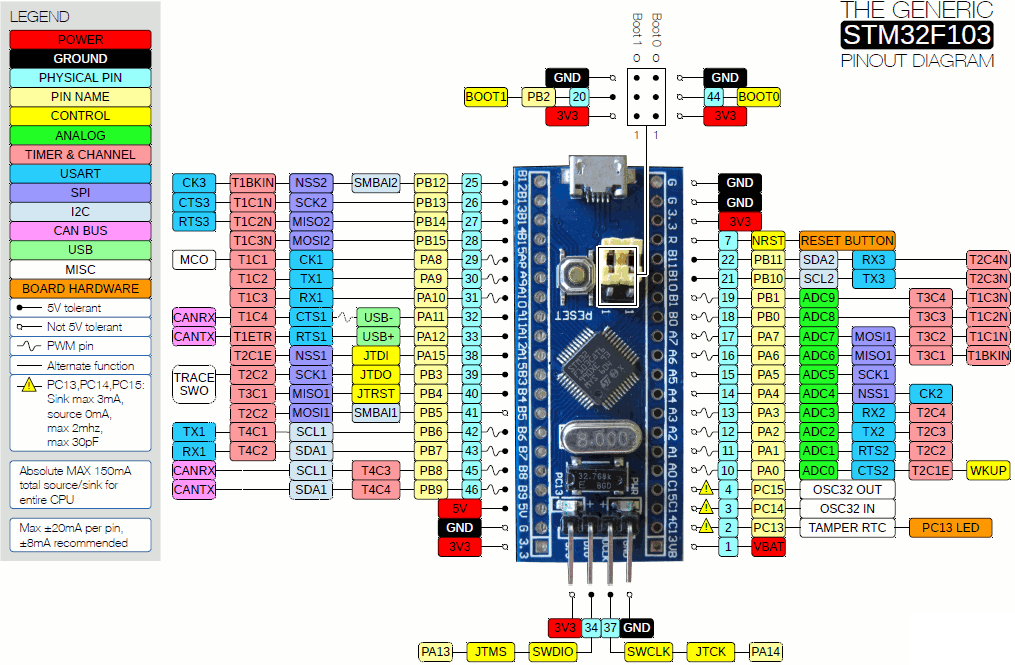
\includegraphics[width=1.0\textwidth]{figures/stm32f1_pinout}
	\caption{Diagrama de pinos do STM32F103C8}
\end{figure}

